\chapter{Introduction}

\section{CubeSat}
A CubSat is a satellite that follows the CubSat standard. The standard was initial developed in a collaboration between California Polytechnic State University and Stanford University with the goal of giving the scientific community affordable aces to space. 

It achieves this by enforcing a strict form factor on the satellite. This gives several advantages, one is that it allows for mass production of components as everybody follows the same standard. It also means that the process of finding a launch provider is a lot easier. As they all have the same form factor, standardized launch interfaces have been created and even the ISS has the opportunity to launch CubSats. 

The most important part of the specification is the size and mass. CubeSats can come in different sizes but they are all based on the 'unit' called 1U. A 1U is 10x10x10cm cube that has a mass of no more than \SI{1.33}{\kilogram}. You can get different sizes by staking 1Us together. Normal sizes are 1U, 2U,3U and 6U. The limit in size and mass heavily influences the design and means you very often are working with limited battery capacity. It also affect the attitude determination and control system(ADCS) as it becomes difficult to add truster and adding reaction wheels become a big cost as they take up a lot of space and mass\cite{CubeSat101}.                         

\section{The MOVE-II CubeSat}
The MOVE-II CubeSat is a 1U CubeSat. It is a project at the Lehrstuhls f�r Raumfahrttechnik(LRT) whit support from Deutsche Luft- und Raumfahrtzentrum(DLR) and in cooperation with the Wissenschaftlichen Arbeeitsgemenschaft f�r Raketentechnik und Raumfahrt(WARR). 


\ifdraft
The MOVE-II CubeSat consists primarily of seven subsystems. 

\subsubsection{Thermal}
The Thermal subsystem is in charge of monitoring the temperature of satellite and make sure that it does not overheat. It was also a big part in the design to make sure there where no parts that is designed in such a way that they produce to much heat. 

\subsubsection{Communication}
The communication subsystem has the responsibility of the radio communication between the satellite a and the ground station. The satellite is equipped with a UHF/VHF antenna and and S-Band antenna. 

\subsubsection{Computer data handler}
works as the main      
\fi

Most of the students working on the project are volunteers. As the development face of the project is ending whit the planed launch in October the number of active students is going down but at the most there was over a 100 students working on the project. There is still a lot of work that can be done on the project, even if the satellite is launching in October. Both in therms of data analysis and future development of software as most of the software can be updated once the satellite is in orbit. 

This is especially true for the ADCS as it generates a lot of sensor data and there are many parts of the software that can be improved. One of these improvements for the ADCS is to activate the extended Kalman filter(EKF). The EKF was not sufficiently tested before the launch software was frozen so it is not a part of the launch. At a later time and as a part of this rapport significant effort has been put into testing the EKF so it can be implemented as soon as the projects open up for uploading new software to the satellite.               

\section{Attitude Determination and Control System}
The attitude determination and control system (ADCS) of a satellite has the task of determining and controlling the attitude of the satellite. For the MOVE-II mission it is required that the top panel of the satellite is pointing towards the sun. There are two main reasons for this. The first is that the payload requires sun pointing. The experimental solar cells that are the payload of the MOVE-II CubeSat are positioned on the top panel of the satellite. They require to be in the sun so their efficiency can be measured. The second reason is that the satellite has four flap panels that will be deployed after launch to a position where they creates a large area of solar cells with the top panel see \autoref{fig:Sat_Deployed}. So to maximize the energy generated by the solar cells they should be facing the sun.

\begin{figure}[tbp]
	\centering
	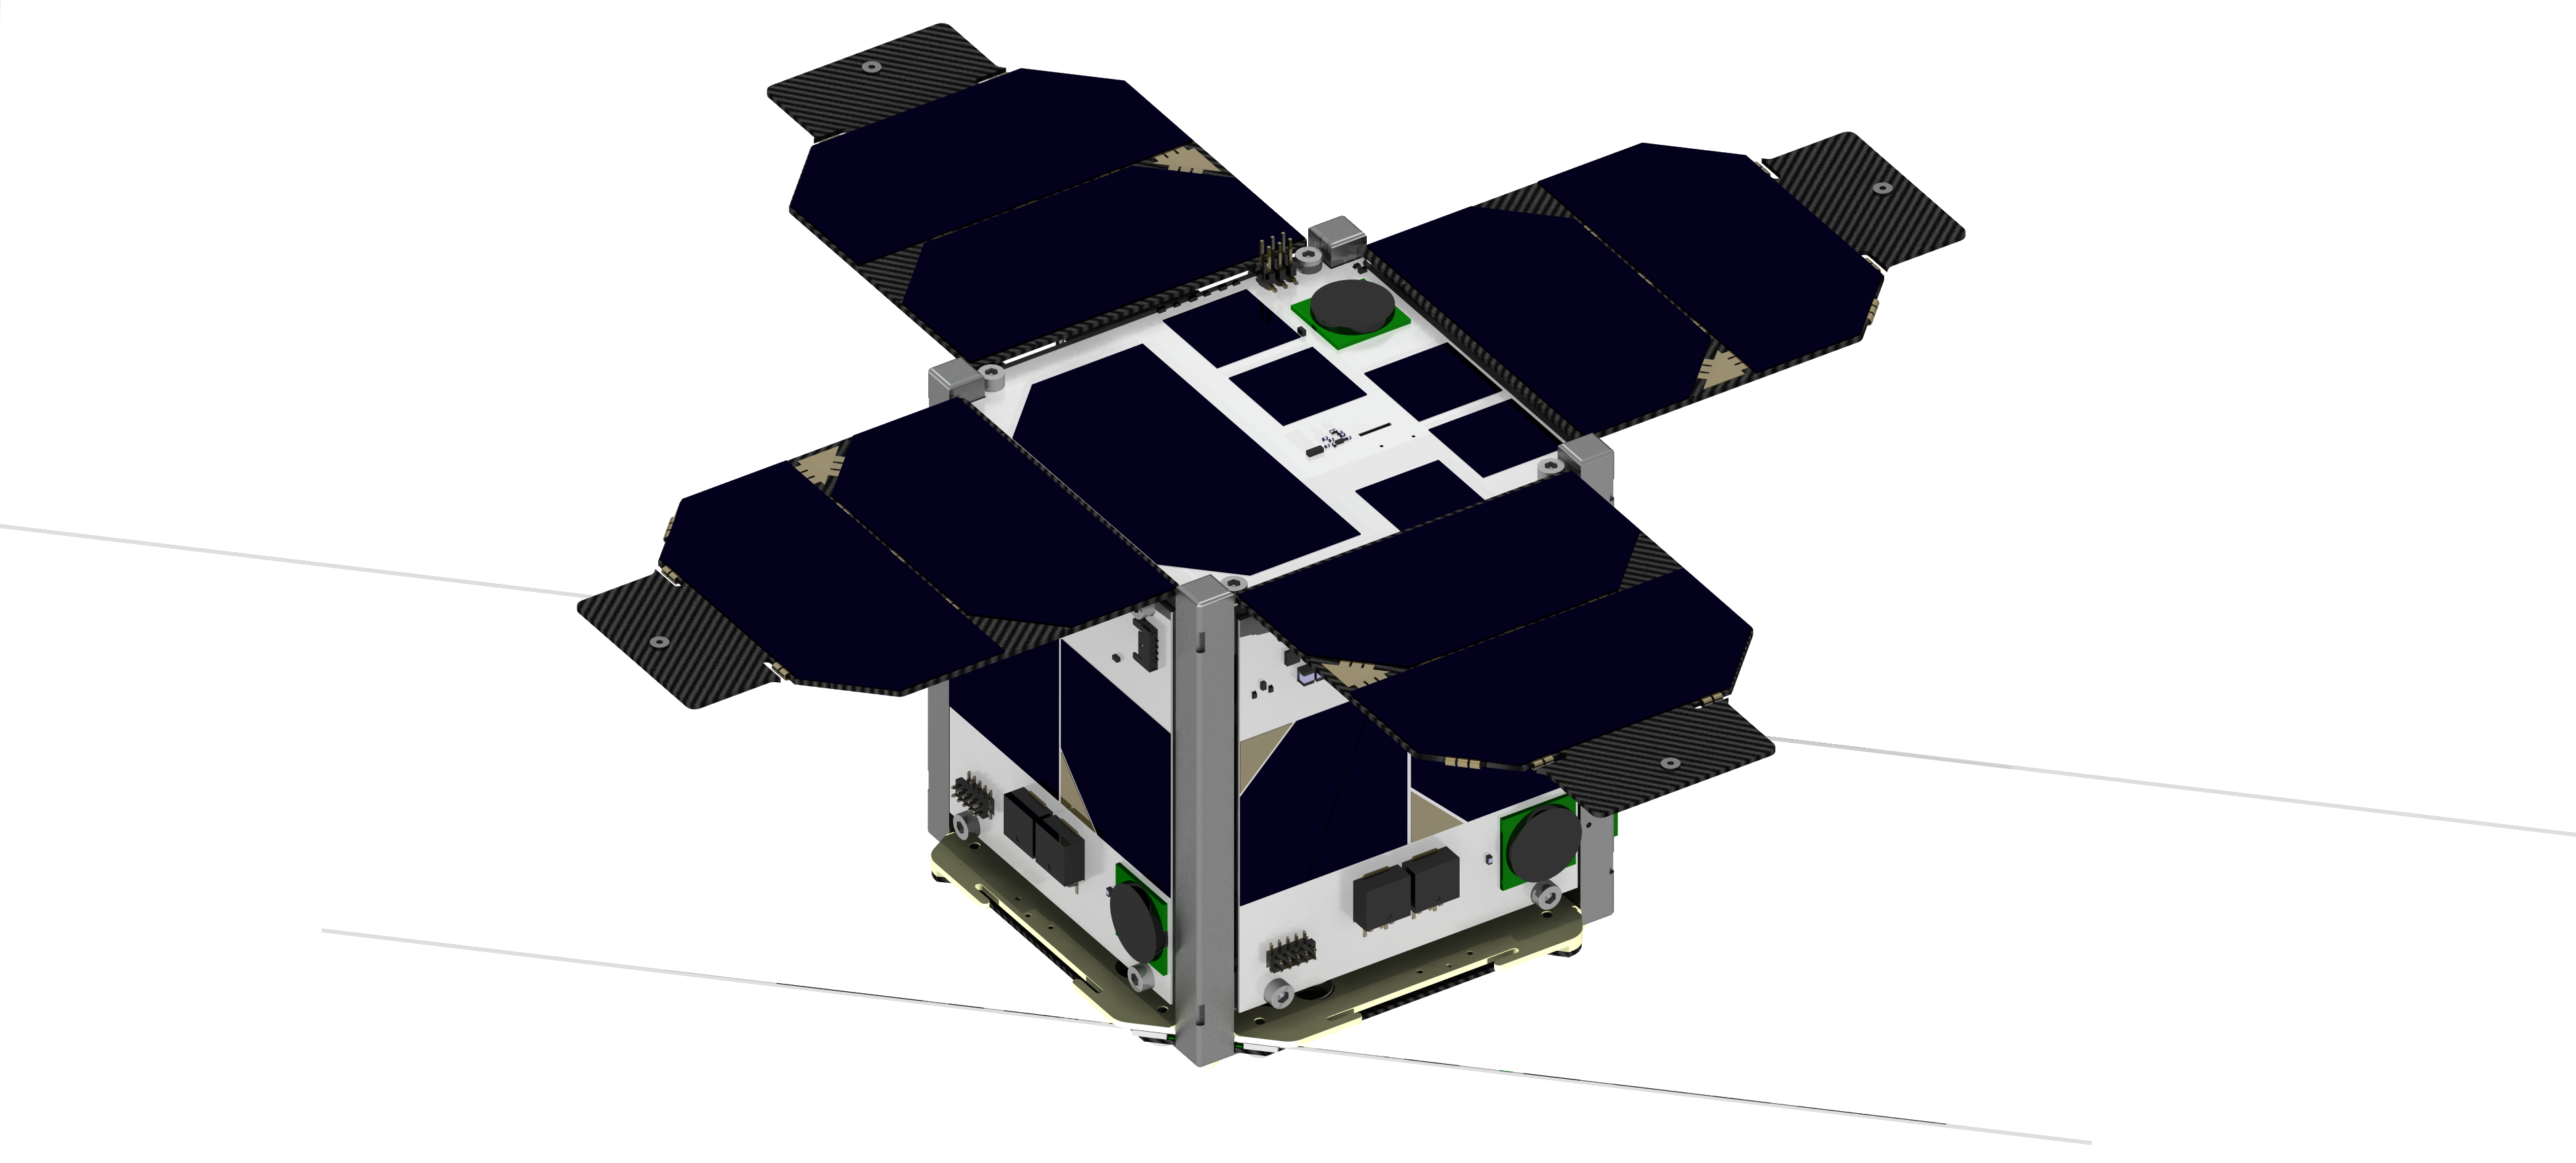
\includegraphics[width=\linewidth,scale=1]{./Pictures/SatelliteDeployed}
	\caption{Rendering of the MOVE-II CubeSat with flap panels deployed}
	\label{fig:Sat_Deployed}
\end{figure}

The ADCS is normally a complex system that can be designed in many different ways. In general on a high level the ADCS can be described as a classical control system consisting of a control component, actuator component and sensor component creating a closed loop control system. There might also be observers or estimators either to use the estimates in the controller or for simply recording the estimated position of the satellite. The normal actuators for satellites are coils interacting with the magnetic felled of the earth to create a torque see \autoref{eq:Mag_Control} \cite[p.~295]{move-ii-sysdoc}, reaction whiles or thrusters. For the CubSats the most common is magnetic coils and sometimes reaction whiles. Thrusters are very rarely used. The sensor can consists of many different sensors and it is very common to combine several types of sensors. Common sensors include magnetometers to measure the magnetic felled of the earth. Light sensors often named sun sensors that measure light intensities and can be used to determine the direction of the sun. Gyroscopes to measure the rotation of the satellite. If estimators are used the sensor data is very often used in combination with models of the sun position and models of the magnetic felled.                    

\begin{equation}\label{eq:Mag_Control}
	\vec{T} = \vec{M} \times \vec{B}
\end{equation}

\subsection{MOVE-II ADCS Architecture}
The adcs for MOVE-II consists of six panels see \autoref{fig:ADCS_panel_overwive} for placement in satellite. Each having a micro-controller, BMX sensor, coils and a sun sensor except for the main panel that does not have a sun sensor. The BMX sensor is a combined accelerometer, gyroscope, magnetometer and temperature sensor. The task of the micro-controllers that are not on the main panel is mainly to collect sensor data and control their respective coils. The micro-controller on the main panel also collects sensor data and controls it`s coils. In addition it is ruining the control algorithm, EKF, all the models that are required for the EKF and it communicates with the rest of the satellite. The EKf will be described in more detail in \autoref{chap:EKF}. The main panel gets all the sensor data from the rest of the panels and based on this the control algorithm calculates the appropriate current for each panel that it sent back to all the other micro-controllers.

\begin{figure}[tbp]
	\centering
	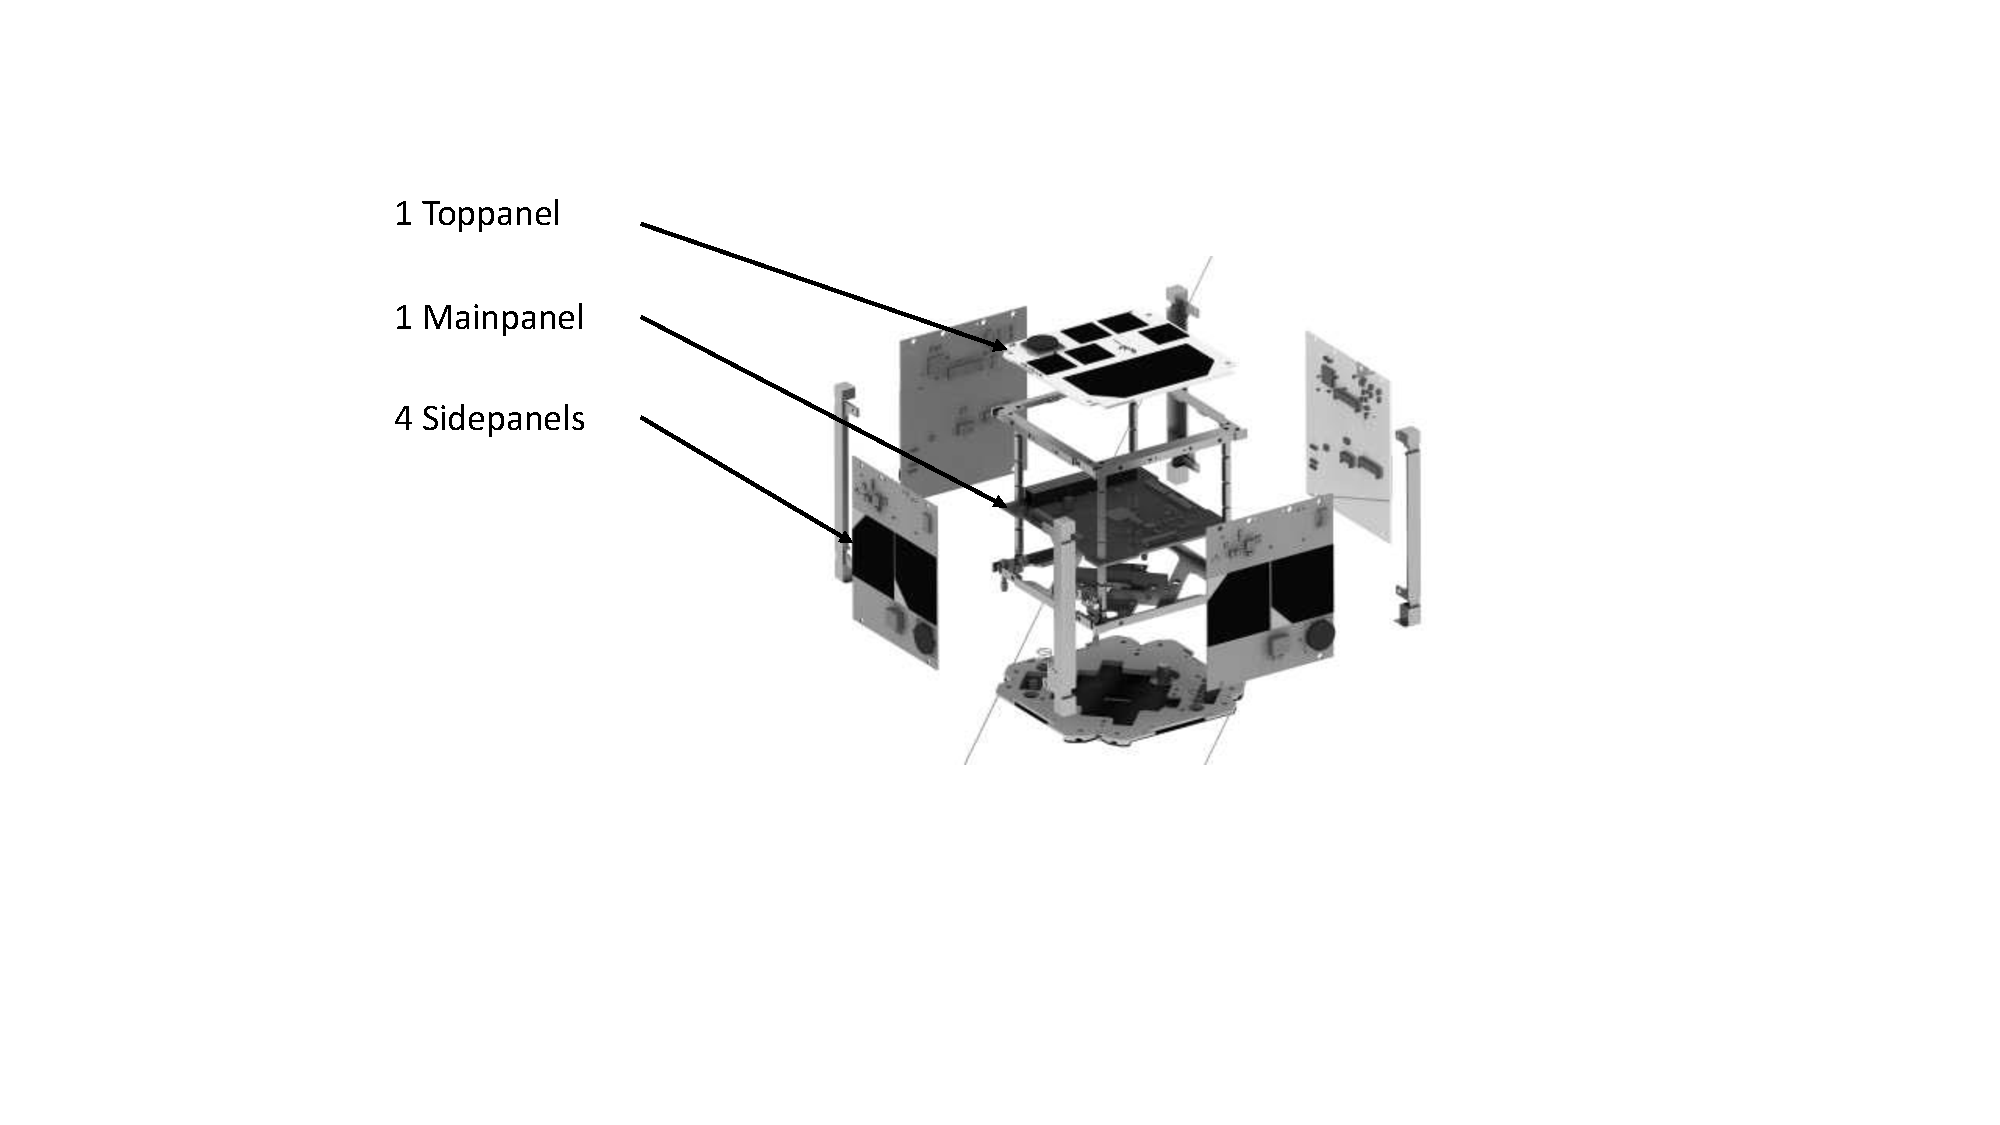
\includegraphics[width=0.8\columnwidth]{./Pictures/ADCSPanels}
	\caption{The placement and name of the different panel of the ADCS}
	\label{fig:ADCS_panel_overwive}
\end{figure}

The ADCS has several modes of operation. The most interesting modes form a attitude control and determination point of we are ATTDET, DETUMB and SUN. For a more in depth view of the different modes of the ADCS see \cite[p.~299]{move-ii-sysdoc}. The ATTDET mode the ADCS calculates the attitude of the satellite and the bias of the gyroscope with a frequency of 5 Hz it does not do any controlling. The attitude and bias is estimated using a EKF. There are many ways of implementing the EKF. For the MOVE-II mission a method where the dynamic model of the satellite is not used, but rather is replaced by gyroscope measurements. For the update step the difference between the sun vector measurements and the sun position and the difference between the magnetometer measurements and the IGRF model is used. 

In the DETUMBL mod the goal is to detumble the satellite down so the satellite can start sun pointing. This mode is intended to be used after the satellite is released from the pod as it is expected to have a high velocity. For this purpose the ADCS uses a bdot controller. The control law can be seen in \autoref{eq:bdot}. Where $\vec{M_ctr}$ is the desired magnetic despoilment, c is the positive constant control gain and $\vec{\dot{B}}$ is the derivative of the measured magnetic in the fixed body frame of the satellite. The control torque is then give by \autoref{eq:Mag_Control}. 

\begin{equation}\label{eq:bdot}
	\vec{M_{ctr}} = -c\vec{\dot{B}}
\end{equation}

In the SUN mode the ADCS tries to point the top panel towards the sun. For this a spinning controller is used with a desired velocity of \SI{5.7}{\degree \per \second} around the z-axis. The spinning sun pointing controller is a state-feedback controller. It has 5 states and the state vector can be seen in \autoref{eq:statevector}. The controller law can be seen in \autoref{eq:control_law}, the controller calculates the desired torque u. As the satellite produces as magnetic moment and not a torque a mapping function \autoref{eq:control_maping} is needed to get $\vec{M_{ctr}}$ \cite[p.~42]{jkiesbyema}. The problem with the spinning controller is that the satellite is not ideal for spinning. The satellite has non diagonal elements on its inertia tensor. This means that the satellite will experience gyroscopic effects when it spines around its z-axis. Compensating for this effects requires actuation witch in turn requires power. This makes the spinning sun pointing controller not very power effective. It is therefore desirable to find a beater and more power efficient controller. On of the suggestions is a controller based on the orientation of the satellite, but for that to be possible the EKF most work.            
 

\begin{align}
	x &= \begin{bmatrix}
    		S_x & S_y & \omega_x & \omega_y & \omega_z 
		 \end{bmatrix}^T \label{eq:statevector}\\
	u &= -Kx\label{eq:control_law}
\end{align} 

\begin{equation}\label{eq:control_maping}
	\vec{M_{ctr}} = \frac{\vec{U} \times \vec{B}}{\mid\vec{B}\mid}
\end{equation}



